\documentclass[11pt, a4paper]{article}
\title{SPS : CW2 Report}
\author{Matthew Duffin}

\renewcommand\thesection{\arabic{section}}
\renewcommand\thesubsection{(\alph{subsection})}

\usepackage[linesnumbered,boxed]{algorithm2e}
\usepackage[margin=2cm]{geometry}
\usepackage{fancyhdr}
\usepackage{graphicx}
\usepackage{subfig}
\usepackage{titling}

\setlength{\droptitle}{-60pt}

\pagestyle{fancy}
\fancyhf{}
\rhead{np14842, md14816}
\lhead{Nick Pearson, Matthew Duffin}
\cfoot{Page \thepage}

\begin{document}
\maketitle

\section{Introduction}
This report describes the steps involved in processing a set of training data with the ultimate goal of creating an accurate classifier. We created two different classifiers using two different techniques. By doing this we gained experience with clustering and classifying data. 

We were provided with two sets of data points. The first contained 150 data points, each with 5 different features. We were not provided with the number of classes that this data had been drawn from. We were also provided with 15 separate data points. These were used to test our classifiers. 

\section{Feature Selection}
Figures ~\ref{fig:feature_matrix} and ~\ref{fig:features_nick} were provided in order to assist us with identifying which two features separate the clusters.

\begin{figure}[ht]
	\centering
	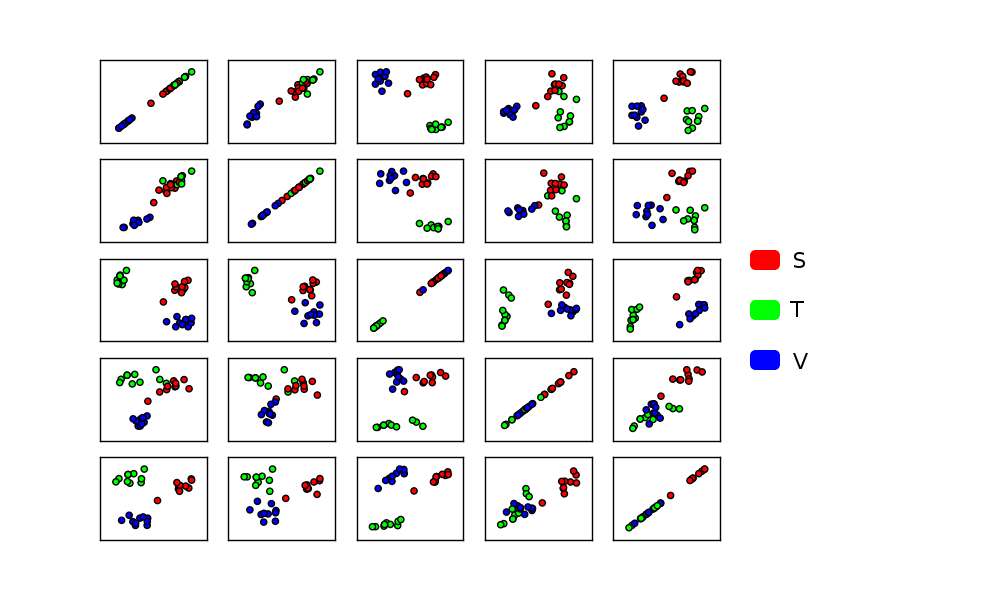
\includegraphics[trim={0 1cm 3cm 1cm},clip,width=0.8\textwidth]{feature_matrix_leg.png}
	\caption{A grid of plots, each of which plots one feature against another.}
	\label{fig:feature_matrix}
\end{figure}

It is immediately obvious that features 2 and 3 on the left, and 2 and 5 on the right, separate the data into three well defined clusters. We then extracted these features and examined them in more detail. You can see the two features plotted against each other in Figures ~\ref{fig:clusters_matt} and ~\ref{fig:clusters_nick}. The inter-cluster distance is high so there is a clear separation between clusters. The intra-cluster distances are low though so the underlying gaussian distributions for each cluster have low variance. 

\section{Class Identification}
During this stage we wanted to derive class labels for each data point. The first method  we used was the K-Means algorithm. At first we ran the algorithm until convergence to ensure that we did not recieve unusual results due to the random nature of initial centroid selection. As you can see from the graph, this worked very well, visually matching our expectations. The K-Means algorithm also returns the inertia. This is the sum of distances of data points to their closest centroid. For Nick's data the value is 163. Given there are 150 data points this means each point is on average roughly 1 unit from the closest centroid, which seems very good. 

%\begin{figure}[ht]
%\centering
%\begin{minipage}[b]{0.45\linewidth}
%	\includegraphics[trim={7cm 0 2cm 0},clip,width=1.1\textwidth]{clusters_matt.pdf}
%	\caption{Matt's data.}
%	\label{fig:clusters_matt}
%\end{minipage}
%%\quad
%\begin{minipage}[b]{0.45\linewidth}
%	\includegraphics[trim={7cm 0 2cm 0},clip,width=1.1\textwidth]{clusters_nick.pdf}
%	\caption{Nick's data.}
%	\label{fig:clusters_nick}
%\end{minipage}
%\end{figure}

% PUT ACTUAL NUMBERS IN ABOVE TEXT

% GRAPH HERE

\subsection{K-Means Experimentation}
The K-Means algorithm has a number of potential flaws. In this part of the coursework we aimed to expose these flaws. K-Means is a heuristic algorithm that finds a local optimum of centroid positions. Therefore there is no guarantee that it will converge to the global optimum \cite{km_wiki}.

%\begin{algorithm}[H]
%
%  \caption{The K-Means algorithm.}
%  \SetKwFunction{algo}{K-Means}
%  \SetKwProg{myalg}{def}{}{}
%  \myalg{\algo{Instances, K}}{
%  randomly initialise vectors $\mu_0$ .. $\mu_K$
%  
%  \Repeat{no change in $\mu_0$ .. $\mu_K$}{
%  	assign each x $\epsilon$ Instances to nearest $\mu$
%  	
%  	re-calculate each $\mu$ as average of points assigned to it
%  	}
%  \Return{$\mu_0$ .. $\mu_K$}
%  }
%\end{algorithm}
Firstly, the algorithm can be given poor choices of initial centroids. You should be able to place two of the initial centroids within one of the clusters so that K-Means splits that cluster in two. The last centroid is then placed between the remaining two clusters so that K-Means treats them as one large cluster. Unfortunately though we were unable to find a configuration where K-Means converged to a non-optimal clustering. 

Next we changed the number of iterations that K-Means went through. The aim here was to cut the algorithm off before it converged. We switched back to random initialisation of centroids and reduced the maximum number of iterations until we saw non-optimal clustering. We found that it was necessary to go all the way down to one or two iterations before non-optimal clustering occurred. This shows that K-Means converges very quickly on these data sets. 

One last way to affect the clustering is to change the distance measure that K-Means uses. Unfortunately we could find no way to do this with the library function that we were using so we couldn't test this option. The algorithm currently uses the Euclidean distance which produces reliable results. If we had managed to change it to the Manhattan distance we may have seen non-optimal clustering.
% GRAPH HERE

\section{Nearest-Centroid Classification}
The next stage of our analysis was to start classifying new data. We started by using the centroids that we found using K-Means as a simple nearest-neighbour classifier. You can see the results in Figures ~\ref{fig:nearest_matt} and ~\ref{fig:nearest_nick}. The crosses represent the test data. As our features had high inter-cluster distance the nearest neighbour produced a fairly good assignment of data points. However, we could not test that it was getting the right result every time as we did not know which cluster each test point was \textit{supposed} to belong to.

%\begin{figure}[ht]
%\centering
%\begin{minipage}[b]{0.45\linewidth}
%	\includegraphics[trim={7cm 0 2cm 0},clip,width=1.1\textwidth]{nearest_matt.pdf}
%	\caption{Matt's data.}
%	\label{fig:nearest_matt}
%\end{minipage}
%%\quad
%\begin{minipage}[b]{0.45\linewidth}
%	\includegraphics[trim={7cm 0 2cm 0},clip,width=1.1\textwidth]{nearest_nick.pdf}
%	\caption{Nick's data.}
%	\label{fig:nearest_nick}
%\end{minipage}
%\end{figure}

% do you have any more to say here
%GRAPH HERE



\section{Maximum-Likelihood Classification}
Next we used a different classification method: maximum-likelihood classification (with each class modelled as being drawn from a 2-D Normal Distribution). This method has certain advantages over nearest-neighbour classification. In ML classification we need to estimate mean vectors as well as full covariance matrices for each class. This may result in a non-linear decision boundary if the covariance matrices are not the same across classes. \nocite{ml_wiki} \nocite{mvn_wiki}

Our first task was to plot contours around each cluster such that 95\% of the probability mass was inside the contour. We did this by finding the points where the squared Mahalanobis distance from the mean was 6. The Mahalanobis distance is a multi-dimensional measurement of how many standard deviations a point is from the mean \cite{mal_wiki}.

Next we plotted the decision boundaries. These allow us to classify future data as belonging to one of the three clusters. To generate these boundaries we found the points where the probabilities of belonging to cluster A's distribution and cluster B's distribution were equal.

%\begin{figure}[ht]
%\centering
%\begin{minipage}[b]{0.45\linewidth}
%	\includegraphics[trim={6cm 0 2cm 0},clip,width=1.1\textwidth]{contour_matt.pdf}
%	\caption{Matt's data.}
%	\label{fig:minipage7}
%\end{minipage}
%%\quad
%\begin{minipage}[b]{0.45\linewidth}
%	\includegraphics[trim={6cm 0 2cm 0},clip,width=1.1\textwidth]{contour_nick.pdf}
%	\caption{Nick's data.}
%	\label{fig:minipage8}
%\end{minipage}
%%\caption{The 15 test data points have been classified. They are shown by an 'x' and the training data by an 'o'.}
%\end{figure}

We then considered how you could change the maximum-likelihood classifier so that its decision boundaries were the same as the ones we found using the nearest-centroid method. We found that you can use the identity matrix as the covariance matrix for the two distributions instead of thier true covariances. This way there appears to be no correlation between the features within each cluster. Also, the two covariance matrices are identical. This creates a straight decision boundary that bisects the line between the two centroids.

%\begin{figure}[ht]
%\centering
%\begin{minipage}[b]{0.45\linewidth}
%	\includegraphics[trim={7cm 0 2cm 0},clip,width=1.1\textwidth]{prior_matt.pdf}
%	\caption{Matt's data.}
%	\label{fig:prior_matt}
%\end{minipage}
%%\quad
%\begin{minipage}[b]{0.45\linewidth}
%	\includegraphics[trim={7cm 0 2cm 0},clip,width=1.1\textwidth]{prior_nick.pdf}
%	\caption{Nick's data.}
%	\label{fig:prior_nick}
%\end{minipage}
%\end{figure}

We also experimented with adding a prior to one of the three classes. Figures ~\ref{fig:prior_matt} and ~\ref{fig:prior_nick} show how the decision boundaries change (dotted line) when one of the classes is twice as likely.

\section{Discussion}
In conclusion, we agreed that the decision boundaries we achieved would be sufficient to assign new data points to our clusters. The use of Maximum-Likelihood Classification would seem more accurate for deciding points which are near the decision boundary, as our clusters had different covariance values from one another. \\
The data we were given demonstrates how much information you can gain without any prior knowledge of where data was sourced. If we had more knowledge we could have used a MAP estimation for a final stage allowing for better results. However, we found that even giving one class a prior of 2 times the rest did not move the decision boundaries very far. This indicates that only a strong prior would affect classification greatly.

\section{Sources}
\renewcommand{\refname}{\vspace{-2em}}
\begin{thebibliography}{9}

\bibitem{mal_wiki}
  Mahalanobis Distance Wikipedia,
  https://en.wikipedia.org/wiki/Mahalanobis\_distance,
  Retrieved 11th March 2016.
  
\bibitem{ml_wiki}
  Maximum Likelihood Wikipedia,
  https://en.wikipedia.org/wiki/Maximum\_likelihood,
  Retrieved 11th March 2016.
  
\bibitem{mvn_wiki}
  Multivariate Normal Wikipedia,
  https://en.wikipedia.org/wiki/Multivariate\_normal\_distribution,
  Retrieved 11th March 2016.
  
\bibitem{km_wiki}
  K-Means Wikipedia,
  https://en.wikipedia.org/wiki/K-means\_clustering,
  Retrieved 11th March 2016.

\end{thebibliography}
\end{document}